\cleardoublepage
\chapter{Discussion}
\label{ch:discussion}

In this section, we provide further insights into the trade-offs observed across the evaluated language-agent architectures.

% ===== Data =====
% ColBERTV2 (k=100)
\pgfplotstableread[row sep=\\,col sep=&]{
dataset & input & output \\
LoCoMo    & 9491602 & 12756 \\
HotpotQA  & 98203664 & 34680 \\
2Wiki     & 173622051 & 55316 \\
MuSiQue   & 30743225 & 10912 \\
}\zsdata

% QA Agent
\pgfplotstableread[row sep=\\,col sep=&]{
dataset & input & output \\
LoCoMo    & 914837 & 786736 \\
HotpotQA  & 5399024 & 4041931 \\
2Wiki     & 10032591 & 6308479 \\
MuSiQue   & 1860903 & 3282503 \\
}\cbdata

% Auto DAG Agent
\pgfplotstableread[row sep=\\,col sep=&]{
dataset & input & output \\
LoCoMo    & 25991129 & 1052529 \\
HotpotQA  & 175128399 & 6775930 \\
2Wiki     & 337343379 & 11912993 \\
MuSiQue   & 84899504 & 2828011 \\
}\hrdata

% Cognitive Agent
\pgfplotstableread[row sep=\\,col sep=&]{
dataset & input & output \\
LoCoMo    & 8199579 & 352909 \\
HotpotQA  & 97289117 & 1876576 \\
2Wiki     & 333623487 & 3722927 \\
MuSiQue   & 67000951 & 955168 \\
}\caData

% ===== Plot style =====
\pgfplotsset{
  qacoststyle/.style={
    ybar stacked,
    bar width=.5cm,
    width=\textwidth,
    height=.5\textwidth,
    grid=major,
    axis line style={draw=none},
    tick label style={font=\scriptsize},
    label style={font=\scriptsize},
    symbolic x coords={LoCoMo,HotpotQA,2Wiki,MuSiQue},
    xtick=data,
    enlarge x limits=0.15,
    nodes near coords,
    nodes near coords align={vertical},
    every node near coord/.append style={
      text=black,
      font=\tiny,
      rotate=90,
      anchor=west,
    },
    ymin=0, ymax=400000000,
    ylabel={Total $token$ consumption},
  }
}

% ===== Figure =====
\begin{figure}[ht]
    \centering
    \begin{tikzpicture}
    
    % ColBERTV2
    \begin{axis}[
        qacoststyle,
        hide axis,
        every node near coord/.append style={yshift=0.75cm}
    ]
    \addplot+[
        nodes near coords=,
        bar shift=-0.75cm,
        fill={rgb,255:red,130; green,130; blue,180}, draw=none,
    ] table[x=dataset, y=input]{\zsdata};
    \addplot+[
        bar shift=-0.75cm,
        fill={rgb,255:red,170; green,170; blue,210}, draw=none,
    ] table[x=dataset, y=output]{\zsdata};
    \end{axis}

    % QA Agent
    \begin{axis}[
        qacoststyle,
        every node near coord/.append style={yshift=0.25cm}
    ]
    \addplot+[
        nodes near coords=,
        bar shift=-0.25cm,
        fill={rgb,255:red,100; green,190; blue,130}, draw=none,
    ] table[x=dataset, y=input]{\cbdata};
    \addplot+[
        bar shift=-0.25cm,
        fill={rgb,255:red,160; green,210; blue,150}, draw=none,
    ] table[x=dataset, y=output]{\cbdata};
    \end{axis}

    % Auto DAG Agent
    \begin{axis}[
        qacoststyle,
        every node near coord/.append style={yshift=-0.25cm}
    ]
    \addplot+[
        nodes near coords=,
        bar shift=0.25cm,
        fill={rgb,255:red,230; green,140; blue,70}, draw=none,
    ] table[x=dataset, y=input]{\hrdata};
    \addplot+[
        bar shift=0.25cm,
        fill={rgb,255:red,250; green,170; blue,100}, draw=none,
    ] table[x=dataset, y=output]{\hrdata};
    \end{axis}

    % Cognitive Agent
    \begin{axis}[
        qacoststyle,
        every node near coord/.append style={yshift=-0.75cm}
    ]
    \addplot+[
        nodes near coords=,
        bar shift=0.75cm,
        fill={rgb,255:red,180; green,90; blue,200}, draw=none,
    ] table[x=dataset, y=input]{\caData};
    \addplot+[
        bar shift=0.75cm,
        fill={rgb,255:red,210; green,130; blue,230}, draw=none,
    ] table[x=dataset, y=output]{\caData};
    \end{axis}

    % ===== Legend =====
    \node[anchor=south, yshift=1.75em] at (current axis.north) {
        \begin{tikzpicture}[baseline]
            \node[
                fill=white,
                draw=gray!50,
                rounded corners=2pt,
                inner sep=4pt
            ] {
                \shortstack{
                    \begin{tabular}{@{}c@{\hskip 0.5em}c@{\hskip 1.5em}c@{\hskip 0.5em}c@{\hskip 1.5em}c@{\hskip 0.5em}c@{\hskip 1.5em}c@{\hskip 0.5em}c@{}}
                        \tikz \draw[fill={rgb,255:red,130; green,130; blue,180}, draw=none] (0,0) rectangle (0.4cm,0.2cm); & \scriptsize ColBERTV2 (k=100) &
                        \tikz \draw[fill={rgb,255:red,100; green,190; blue,130}, draw=none] (0,0) rectangle (0.4cm,0.2cm); & \scriptsize QA Agent &
                        \tikz \draw[fill={rgb,255:red,230; green,140; blue,70}, draw=none] (0,0) rectangle (0.4cm,0.2cm); & \scriptsize Auto DAG Agent &
                        \tikz \draw[fill={rgb,255:red,180; green,90; blue,200}, draw=none] (0,0) rectangle (0.4cm,0.2cm); & \scriptsize Long-lived QA Agent \\
                    \end{tabular}
                    \\
                    {\tiny \textit{Darker shades correspond to input tokens, while lighter shades to output tokens}}
                }
            };
        \end{tikzpicture}
    };

    \end{tikzpicture}
    \caption{Total token usage between ColBERTv2 (k=100), QA Agent, Auto DAG Agent, and Long-lived QA Agent with GPT-4o-mini on the four QA datasets. Darker shades correspond to input tokens, while lighter shades to output tokens.}
    \label{fig:qa_token_prompt_tech}
\end{figure}





\noindent To better understand their computational efficiency, we analyze the total token consumption, separating input and output tokens. Figure \ref{fig:qa_token_prompt_tech} and \ref{fig:qa_avg_token_prompt_tech} present the total and average token usage across the RAG baseline with ColBERTv2 ($k=100$), the QA Agent, the Auto DAG Agent, and the Cognitive QA Agent, evaluated on the four QA datasets, respectively. This comparison shows that more advanced language-agent architectures, particularly those with cognitive features, consume substantially more tokens than simpler baselines. 

\noindent Overall, the simpler QA Agent achieves the best balance between performance and cost. It consumes considerably fewer tokens than one of the strongest RAG baselines, ColBERTv2 ($k = 100$), while delivering results that remain competitive with more advanced language-agent architectures such as the Auto DAG Agent. The increased token usage of the Auto DAG Agent arises from the expansion of its working memory, which accumulates contextual information as it advances through the reasoning plan. Moreover, its procedural memory requires additional space to encode the rules that govern internal actions and updates to its episodic memory, including few-shot examples.

\noindent Similarly, the Long-lived QA Agent exhibits higher token consumption, particularly on 2Wiki and MuSiQue, where it also achieves strong performance. In these cases, the agent retrieves and integrates a larger number of semantically related examples from its long-term memory, increasing input tokens counts.

% ===== Data =====
% ColBERTV2 (k=100)
\pgfplotstableread[row sep=\\,col sep=&]{
dataset & input & output \\
LoCoMo    & 6236.3 & 8.4 \\
HotpotQA  & 13303.4 & 4.6 \\
2Wiki     & 13816.4 & 4.4 \\
MuSiQue   & 12735.4 & 4.5 \\
}\zsdata

% QA Agent
\pgfplotstableread[row sep=\\,col sep=&]{
dataset & input & output \\
LoCoMo    & 3373.4 & 116.8 \\
HotpotQA  & 5016.2 & 154.0 \\
2Wiki     & 7081.5 & 191.1 \\
MuSiQue   & 10582.4 & 256.7 \\
}\cbdata

% Auto DAG Agent
\pgfplotstableread[row sep=\\,col sep=&]{
dataset & input & output \\
LoCoMo    & 17043.4 & 690.2 \\
HotpotQA  & 23650.0 & 915.0 \\
2Wiki     & 26824.4 & 947.3 \\
MuSiQue   & 35126.0 & 1170.1 \\
}\hrdata

% Cognitive Agent
\pgfplotstableread[row sep=\\,col sep=&]{
dataset & input & output \\
LoCoMo    & 5376.8 & 231.4 \\
HotpotQA  & 13138.3 & 253.4 \\
2Wiki     & 26528.6 & 296.0 \\
MuSiQue   & 27720.7 & 395.2 \\
}\caData

% ===== Plot style =====
\pgfplotsset{
  qacoststyle/.style={
    ybar stacked,
    bar width=.5cm,
    width=\textwidth,
    height=.5\textwidth,
    grid=major,
    axis line style={draw=none},
    tick label style={font=\scriptsize},
    label style={font=\scriptsize},
    symbolic x coords={LoCoMo,HotpotQA,2Wiki,MuSiQue},
    xtick=data,
    enlarge x limits=0.15,
    nodes near coords,
    nodes near coords align={vertical},
    every node near coord/.append style={
      text=black,
      font=\tiny,
      rotate=90,
      anchor=west,
    },
    ymin=0, ymax=45000,
    ylabel={Average $token$ consumption},
  }
}

% ===== Figure =====
\begin{figure}[ht]
    \centering
    \begin{tikzpicture}
    
    % ColBERTV2
    \begin{axis}[
        qacoststyle,
        hide axis,
        every node near coord/.append style={yshift=0.75cm}
    ]
    \addplot+[
        nodes near coords=,
        bar shift=-0.75cm,
        fill={rgb,255:red,130; green,130; blue,180}, draw=none,
    ] table[x=dataset, y=input]{\zsdata};
    \addplot+[
        bar shift=-0.75cm,
        fill={rgb,255:red,170; green,170; blue,210}, draw=none,
    ] table[x=dataset, y=output]{\zsdata};
    \end{axis}

    % QA Agent
    \begin{axis}[
        qacoststyle,
        every node near coord/.append style={yshift=0.25cm}
    ]
    \addplot+[
        nodes near coords=,
        bar shift=-0.25cm,
        fill={rgb,255:red,100; green,190; blue,130}, draw=none,
    ] table[x=dataset, y=input]{\cbdata};
    \addplot+[
        bar shift=-0.25cm,
        fill={rgb,255:red,160; green,210; blue,150}, draw=none,
    ] table[x=dataset, y=output]{\cbdata};
    \end{axis}

    % Auto DAG Agent
    \begin{axis}[
        qacoststyle,
        every node near coord/.append style={yshift=-0.25cm}
    ]
    \addplot+[
        nodes near coords=,
        bar shift=0.25cm,
        fill={rgb,255:red,230; green,140; blue,70}, draw=none,
    ] table[x=dataset, y=input]{\hrdata};
    \addplot+[
        bar shift=0.25cm,
        fill={rgb,255:red,250; green,170; blue,100}, draw=none,
    ] table[x=dataset, y=output]{\hrdata};
    \end{axis}

    % Cognitive Agent
    \begin{axis}[
        qacoststyle,
        every node near coord/.append style={yshift=-0.75cm}
    ]
    \addplot+[
        nodes near coords=,
        bar shift=0.75cm,
        fill={rgb,255:red,180; green,90; blue,200}, draw=none,
    ] table[x=dataset, y=input]{\caData};
    \addplot+[
        bar shift=0.75cm,
        fill={rgb,255:red,210; green,130; blue,230}, draw=none,
    ] table[x=dataset, y=output]{\caData};
    \end{axis}

    % ===== Legend =====
    \node[anchor=south, yshift=1.75em] at (current axis.north) {
        \begin{tikzpicture}[baseline]
            \node[
                fill=white,
                draw=gray!50,
                rounded corners=2pt,
                inner sep=4pt
            ] {
                \shortstack{
                    \begin{tabular}{@{}c@{\hskip 0.5em}c@{\hskip 1.5em}c@{\hskip 0.5em}c@{\hskip 1.5em}c@{\hskip 0.5em}c@{\hskip 1.5em}c@{\hskip 0.5em}c@{}}
                        \tikz \draw[fill={rgb,255:red,130; green,130; blue,180}, draw=none] (0,0) rectangle (0.4cm,0.2cm); & \scriptsize ColBERTv2 (k=100) &
                        \tikz \draw[fill={rgb,255:red,100; green,190; blue,130}, draw=none] (0,0) rectangle (0.4cm,0.2cm); & \scriptsize QA Agent &
                        \tikz \draw[fill={rgb,255:red,230; green,140; blue,70}, draw=none] (0,0) rectangle (0.4cm,0.2cm); & \scriptsize Auto DAG Agent &
                        \tikz \draw[fill={rgb,255:red,180; green,90; blue,200}, draw=none] (0,0) rectangle (0.4cm,0.2cm); & \scriptsize Long-lived QA Agent \\
                    \end{tabular}
                    \\
                    {\tiny \textit{Darker shades correspond to input tokens, while lighter shades to output tokens}}
                }
            };
        \end{tikzpicture}
    };

    \end{tikzpicture}
    \caption{Average token usage between ColBERTv2 (k=100), QA Agent, Auto DAG Agent, and Long-lived QA Agent with GPT-4o-mini on the four QA datasets. Darker shades correspond to input tokens, while lighter shades to output tokens.}
    \label{fig:qa_avg_token_prompt_tech}
\end{figure}





\noindent These findings highlight a key challenge for the broader adoption of language-agent architectures in QA systems. The substantial token overhead not only raises inference costs but also introduces additional latency, posing further challenges for scalable applications.

\noindent Furthermore, Figure \ref{fig:locomo_dist} shows the distribution of questions with $R_1 < 0.5$ in the LoCoMo dataset for the strongest baseline, RAG with ColBERTv2 ($k = 100$), and the Auto DAG Agent with GPT-4o-mini. Single-hop questions account for $43.9\%$ of incorrect questions for ColBERTv2 and $51.7\%$ for the Auto DAG Agent, showing that the language agent struggles to generalize to different question types. We also observe an increase in the number of multi-hop questions answered incorrectly by the agent, but these questions have a different structure compared to other datasets. For example, the question \textit{Where has Melanie camped?} requires gathering information from multiple conversations turns to provide the expected answer (\textit{beach, mountains, forest}). However, the question is not composed of multiple-sub-questions, a structure that the language agents are specifically designed to handle, which helps explain the drop in performance on this benchmark.

\begin{figure}[h]
    \centering
    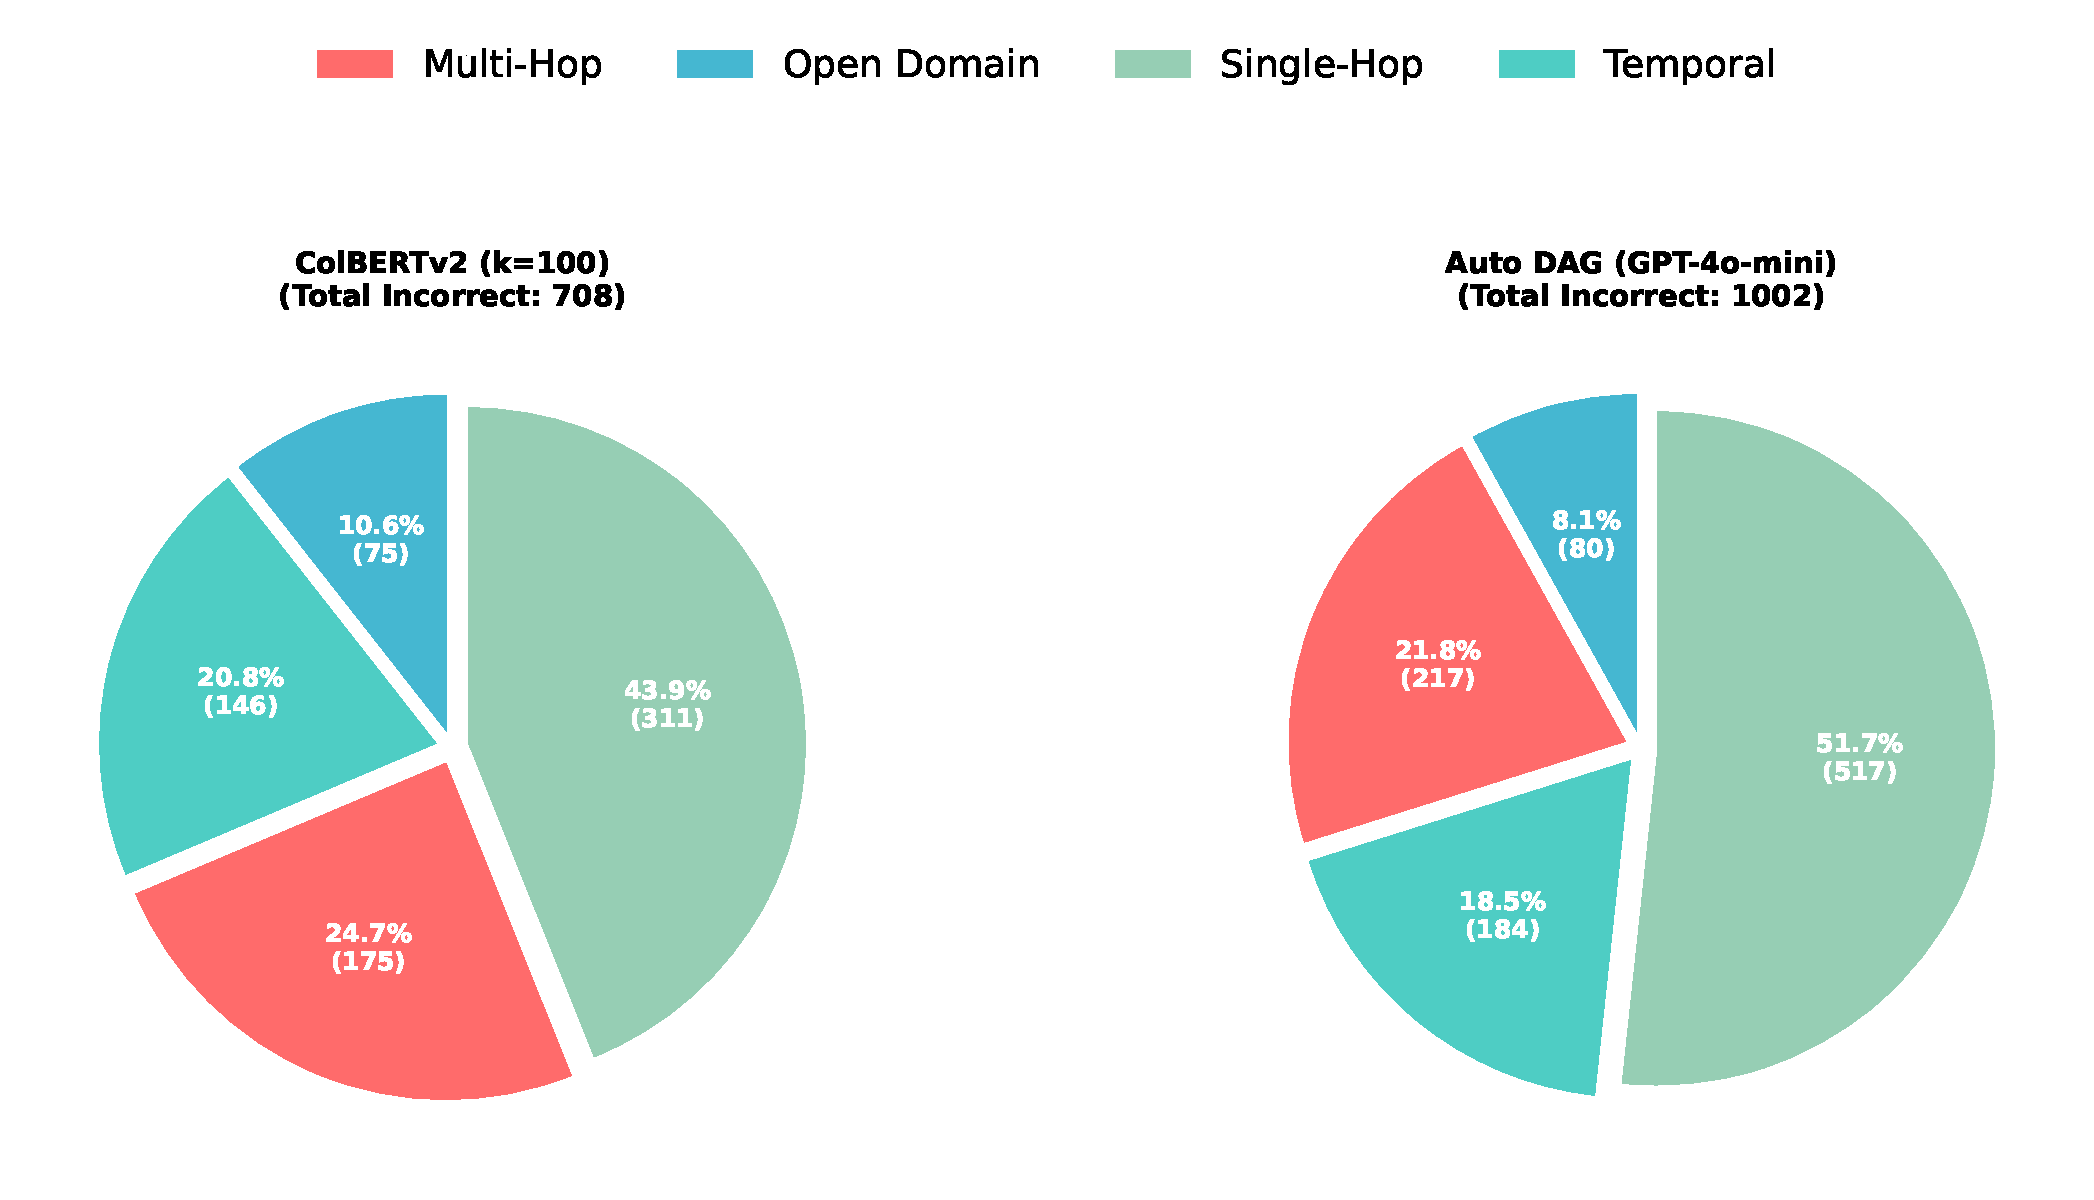
\includegraphics[width=.9\textwidth]{images/locomo_error_comparison.eps}
    \caption{LoCoMo error distribution between ColBERTv2 ($k = 100$) and Auto DAG Agent with GPT-4o-mini.}
    \label{fig:locomo_dist}
\end{figure}